%%%%%%%%%%%%%%%%%%%%%%%%%%%%%%%%%%%%%%%%%%%%%%%%%%%%%%%%%%%%%%%%%%%%%%%%%%%%%%%%%%%%%%%%%%%%%%%%%
%%%%%  Beamer Slides  %%%%%%%%%%%%%%%%%%%%%%%%%%%%%%%%%%%%%%%%%%%%%%%%%%%%%%%%%%%%%%%%%%%%%%%%%%%
%%%%%%%%%%%%%%%%%%%%%%%%%%%%%%%%%%%%%%%%%%%%%%%%%%%%%%%%%%%%%%%%%%%%%%%%%%%%%%%%%%%%%%%%%%%%%%%%%

% https://en.wikibooks.org/wiki/LaTeX/Presentations

\documentclass{beamer}
% \mode<presentation> {
\mode<handout> {

    %%%%%  Themes  %%%%%%%%%%%%%%
    %%%%%%%%%%%%%%%%%%%%%%%%%%%%%
    % \usetheme{AnnArbor}
    % \usetheme{Antibes}
    % \usetheme{Bergen}
    % \usetheme{Berkeley}
    % \usetheme{Berlin}
    % \usetheme{CambridgeUS}
    % \usetheme{Copenhagen}
    % \usetheme{Darmstadt}
    % \usetheme{Dresden}
    % \usetheme{Frankfurt}
    % \usetheme{Goettingen}
    % \usetheme{Hannover}
    % \usetheme{Ilmenau}
    % \usetheme{JuanLesPins}
    % \usetheme{Luebeck}
    % \usetheme{Madrid}
    % \usetheme{Malmoe}
    % \usetheme{Marburg}
    % \usetheme{Montpellier}
    % \usetheme{PaloAlto}
    % \usetheme{Pittsburgh}
    % \usetheme{Rochester}
    % \usetheme{Singapore}
    % \usetheme{Szeged}
    % \usetheme{Warsaw}
    % \usetheme{boxes}
    \usetheme{default}

    %%%%%  Color Themes  %%%%%%%%
    %%%%%%%%%%%%%%%%%%%%%%%%%%%%%
    % \usecolortheme{default}
    % \usecolortheme{albatross}
    % \usecolortheme{beaver}
    % \usecolortheme{beetle}
    % \usecolortheme{crane}
    % \usecolortheme{dolphin}
    % \usecolortheme{dove}
    % \usecolortheme{fly}
    % \usecolortheme{lily}
    % \usecolortheme{orchid}
    % \usecolortheme{rose}
    % \usecolortheme{seagull}
    % \usecolortheme{seahorse}
    % \usecolortheme{whale}
    % \usecolortheme{wolverine}

    %%%%%  Outer Themes  %%%%%%%%
    %%%%%%%%%%%%%%%%%%%%%%%%%%%%%
    % \useoutertheme{infolines}
    % \useoutertheme{miniframes}
    % \useoutertheme{shadow}
    % \useoutertheme{sidebar}
    % \useoutertheme{smoothbars}
    % \useoutertheme{smoothtree}
    % \useoutertheme{split}
    % \useoutertheme{tree}

    %%%%%  Inner Themes  %%%%%%%%
    %%%%%%%%%%%%%%%%%%%%%%%%%%%%%
    % \useinnertheme{rectangles}
    % \useinnertheme{circles}
    % \useinnertheme{inmargin}
    % \useinnertheme{rounded}
}

\usepackage{amsthm}
\usepackage{amsmath}
\usepackage{amssymb}
\usepackage{array}
\usepackage[fleqn]{mathtools}
\usepackage{caption}
\usepackage{wallpaper}
\usepackage{xcolor}
\definecolor{umblue}{HTML}{00274C}
\definecolor{ummaize}{HTML}{FFCB05}
\usepackage{colortbl}
\usepackage{graphicx}
\usepackage{pgf}
\usepackage{tikz}
\usetikzlibrary{arrows,automata}
\usepackage{url}
\usepackage{hyperref}

\setbeamercolor{frametitle}{fg=umblue}
\setbeamercolor{item projected}{fg=umblue}
\setbeamercolor{title}{fg=umblue}

\setbeamertemplate{footline}[frame number]
\setbeamertemplate{itemize item}{\color{umblue}$\blacktriangleright$}
\setbeamertemplate{itemize subitem}{\color{umblue}$\ast$}

\setbeamerfont*{footline}{family=\sffamily, size=\large}
\usefonttheme[onlymath]{serif}

\beamertemplatenavigationsymbolsempty

\hypersetup{pdfstartview={Fit}}

\newcommand{\XB}{\color{black}}
\newcommand{\XBB}{\color{blue}}
\newcommand{\XV}{\color{violet}}
\newcommand{\XR}{\color{red}}
\newcommand{\XUMB}{\color{umblue}}
\newcommand{\XUMM}{\color{ummaize}}

\newcommand{\ds}{\displaystyle}

% Use pause in math environments
\makeatletter
\renewrobustcmd{\beamer@@pause}[1][]{
  \unless\ifmeasuring@
  \ifblank{#1}
    {\stepcounter{beamerpauses}}
    {\setcounter{beamerpauses}{#1}}
  \onslide<\value{beamerpauses}->\relax
  \fi
}
\makeatother

%%%%%%%%%%%%%%%%%%%%%%%%%%%%%%%%%%%%%%%%%%%%%%%%%%%%%%%%%%%%%%%%%%%%%%%%%%%%%%%%%%%%%%%%%%%%%%%%%
%%%%%  Title Page  %%%%%%%%%%%%%%%%%%%%%%%%%%%%%%%%%%%%%%%%%%%%%%%%%%%%%%%%%%%%%%%%%%%%%%%%%%%%%%
%%%%%%%%%%%%%%%%%%%%%%%%%%%%%%%%%%%%%%%%%%%%%%%%%%%%%%%%%%%%%%%%%%%%%%%%%%%%%%%%%%%%%%%%%%%%%%%%%

%   Update these lines for each presentation.

\title[Short Title]{Long Title}
\author{\XV\textit{\large{\href{https://github.com/USERNAME}{First Last}}}\XB}
\institute[INSTITUTION]{\normalsize{\textit{\href{mailto:you@institution.edu}{you@institution.edu}}}}
% \titlegraphic{\includegraphics[scale=0.5]{path/to/logo.png}}
\date[]{\today}

\begin{document}

\begin{frame}
    \titlepage
\end{frame}


%%%%%%%%%%%%%%%%%%%%%%%%%%%%%%%%%%%%%%%%%%%%%%%%%%%%%%%%%%%%%%%%%%%%%%%%%%%%%%%%%%%%%%%%%%%%%%%%%
%%%%%  Begin Slides  %%%%%%%%%%%%%%%%%%%%%%%%%%%%%%%%%%%%%%%%%%%%%%%%%%%%%%%%%%%%%%%%%%%%%%%%%%%%
%%%%%%%%%%%%%%%%%%%%%%%%%%%%%%%%%%%%%%%%%%%%%%%%%%%%%%%%%%%%%%%%%%%%%%%%%%%%%%%%%%%%%%%%%%%%%%%%%

%%%%%  Introduction  %%%%%%%%%%%%%%%%%%%%%%%%%%%%%%%%%%%%%%%%%%%%%%%%%%%%%%%%%%%%%%%%%%%%%%%%%%%%

\section{Introduction}

\begin{frame}

    \frametitle{Introduction}

    Simple List \pause

    \vspace{2.5mm}
    \begin{itemize}
        \item Item.\pause
        \begin{itemize}
            \item Sub Item.\pause
        \end{itemize}
    \end{itemize}

\end{frame}

%%%%%  Section Name  %%%%%%%%%%%%%%%%%%%%%%%%%%%%%%%%%%%%%%%%%%%%%%%%%%%%%%%%%%%%%%%%%%%%%%%%%%%%

\section{Section Name}

\begin{frame}

    \frametitle{Math Alignment}

    \begin{flalign*}
        & \ds f(x) = x^2 \\ \pause
        &= x \cdot x
    \end{flalign*}

\end{frame}

\begin{frame}

    \frametitle{TikZ Graph}
    \begin{figure}[t]
        \centering
        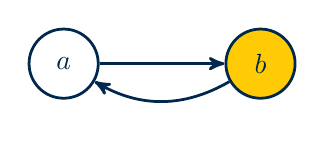
\begin{tikzpicture}[->,>=stealth',auto,node distance=2.5cm,semithick,line width=1pt]
            \tikzstyle{be}=[color=umblue]

            \node[state,fill=white,draw=umblue,text=umblue] (A)              {$a$};
            \node[state,fill=ummaize,draw=umblue,text=umblue] (B) [right of=A] {$b$};

            \path   (A) edge [be] node {} (B)
                    (B) edge [be, bend left] node {} (A);
        \end{tikzpicture}
    \end{figure}

\end{frame}

%%%%%  Conclusion  %%%%%%%%%%%%%%%%%%%%%%%%%%%%%%%%%%%%%%%%%%%%%%%%%%%%%%%%%%%%%%%%%%%%%%%%%%%%%%%

\section{Conclusion}

\begin{frame}
    \frametitle{Conclusion}

    Summary of findings.\pause

    \hrulefill \\
    \Large{\centerline{\XR QUESTIONS?\XB}}
    \normalsize{\centerline{\textit{\href{mailto:you@institution.edu}{you@institution.edu}}}}

\end{frame}

\begin{frame}
    \frametitle{References}

    [1] Author, A. Title. Journal, Year. \\

    [2] Author, B. Title. Conference, Year. \\

\end{frame}

\end{document}
